\documentclass[twoside]{book}

% Packages required by doxygen
\usepackage{calc}
\usepackage{doxygen}
\usepackage{graphicx}
\usepackage[utf8]{inputenc}
\usepackage{makeidx}
\usepackage{multicol}
\usepackage{multirow}
\usepackage{textcomp}
\usepackage[table]{xcolor}

% Font selection
\usepackage[T1]{fontenc}
\usepackage{mathptmx}
\usepackage[scaled=.90]{helvet}
\usepackage{courier}
\usepackage{amssymb}
\usepackage{sectsty}
\renewcommand{\familydefault}{\sfdefault}
\allsectionsfont{%
  \fontseries{bc}\selectfont%
  \color{darkgray}%
}
\renewcommand{\DoxyLabelFont}{%
  \fontseries{bc}\selectfont%
  \color{darkgray}%
}

% Page & text layout
\usepackage{geometry}
\geometry{%
  a4paper,%
  top=2.5cm,%
  bottom=2.5cm,%
  left=2.5cm,%
  right=2.5cm%
}
\tolerance=750
\hfuzz=15pt
\hbadness=750
\setlength{\emergencystretch}{15pt}
\setlength{\parindent}{0cm}
\setlength{\parskip}{0.2cm}
\makeatletter
\renewcommand{\paragraph}{%
  \@startsection{paragraph}{4}{0ex}{-1.0ex}{1.0ex}{%
    \normalfont\normalsize\bfseries\SS@parafont%
  }%
}
\renewcommand{\subparagraph}{%
  \@startsection{subparagraph}{5}{0ex}{-1.0ex}{1.0ex}{%
    \normalfont\normalsize\bfseries\SS@subparafont%
  }%
}
\makeatother

% Headers & footers
\usepackage{fancyhdr}
\pagestyle{fancyplain}
\fancyhead[LE]{\fancyplain{}{\bfseries\thepage}}
\fancyhead[CE]{\fancyplain{}{}}
\fancyhead[RE]{\fancyplain{}{\bfseries\leftmark}}
\fancyhead[LO]{\fancyplain{}{\bfseries\rightmark}}
\fancyhead[CO]{\fancyplain{}{}}
\fancyhead[RO]{\fancyplain{}{\bfseries\thepage}}
\fancyfoot[LE]{\fancyplain{}{}}
\fancyfoot[CE]{\fancyplain{}{}}
\fancyfoot[RE]{\fancyplain{}{\bfseries\scriptsize Generated on Tue Aug 30 2016 11\-:18\-:16 for Client Bluetooth by Doxygen }}
\fancyfoot[LO]{\fancyplain{}{\bfseries\scriptsize Generated on Tue Aug 30 2016 11\-:18\-:16 for Client Bluetooth by Doxygen }}
\fancyfoot[CO]{\fancyplain{}{}}
\fancyfoot[RO]{\fancyplain{}{}}
\renewcommand{\footrulewidth}{0.4pt}
\renewcommand{\chaptermark}[1]{%
  \markboth{#1}{}%
}
\renewcommand{\sectionmark}[1]{%
  \markright{\thesection\ #1}%
}

% Indices & bibliography
\usepackage{natbib}
\usepackage[titles]{tocloft}
\setcounter{tocdepth}{3}
\setcounter{secnumdepth}{5}
\makeindex

% Hyperlinks (required, but should be loaded last)
\usepackage{ifpdf}
\ifpdf
  \usepackage[pdftex,pagebackref=true]{hyperref}
\else
  \usepackage[ps2pdf,pagebackref=true]{hyperref}
\fi
\hypersetup{%
  colorlinks=true,%
  linkcolor=blue,%
  citecolor=blue,%
  unicode%
}

% Custom commands
\newcommand{\clearemptydoublepage}{%
  \newpage{\pagestyle{empty}\cleardoublepage}%
}


%===== C O N T E N T S =====

\begin{document}

% Titlepage & ToC
\hypersetup{pageanchor=false}
\pagenumbering{roman}
\begin{titlepage}
\vspace*{7cm}
\begin{center}%
{\Large Client Bluetooth }\\
\vspace*{1cm}
{\large Generated by Doxygen 1.8.6}\\
\vspace*{0.5cm}
{\small Tue Aug 30 2016 11:18:16}\\
\end{center}
\end{titlepage}
\clearemptydoublepage
\tableofcontents
\clearemptydoublepage
\pagenumbering{arabic}
\hypersetup{pageanchor=true}

%--- Begin generated contents ---
\chapter{Todo List}
\label{todo}
\hypertarget{todo}{}

\begin{DoxyRefList}
\item[\label{todo__todo000001}%
\hypertarget{todo__todo000001}{}%
Class \hyperlink{classAction}{Action} ]Creer une hiérarchie d'actions au lieu d'une seule classe pour tous les types La classe \hyperlink{classAction}{Action} permet de représenter une action élémentaire que le robot doit effectuer  
\item[\label{todo__todo000002}%
\hypertarget{todo__todo000002}{}%
Class \hyperlink{classDevice}{Device} ]Mise à jour du rssi en temps réel Cette classe permet de scanner les devices B\-L\-E 
\end{DoxyRefList}
\chapter{Deprecated List}
\label{deprecated}
\hypertarget{deprecated}{}

\begin{DoxyRefList}
\item[\label{deprecated__deprecated000001}%
\hypertarget{deprecated__deprecated000001}{}%
Class \hyperlink{classDeviceScanner}{Device\-Scanner} ]Effectuer un nouveau scan pour mettre à jour le rssi est lent et nécessite d'être déconnecté 
\end{DoxyRefList}
\chapter{Hierarchical Index}
\section{Class Hierarchy}
This inheritance list is sorted roughly, but not completely, alphabetically\-:\begin{DoxyCompactList}
\item \contentsline{section}{Action}{\pageref{classAction}}{}
\item \contentsline{section}{Analyseur\-Paquet}{\pageref{classAnalyseurPaquet}}{}
\item \contentsline{section}{File}{\pageref{classFile}}{}
\item Q\-Dialog\begin{DoxyCompactList}
\item \contentsline{section}{Ajouter\-Window}{\pageref{classAjouterWindow}}{}
\item \contentsline{section}{Apprendre\-Window}{\pageref{classApprendreWindow}}{}
\end{DoxyCompactList}
\item Q\-Main\-Window\begin{DoxyCompactList}
\item \contentsline{section}{Main\-Window}{\pageref{classMainWindow}}{}
\end{DoxyCompactList}
\item Q\-Object\begin{DoxyCompactList}
\item \contentsline{section}{Device}{\pageref{classDevice}}{}
\item \contentsline{section}{Device\-Scanner}{\pageref{classDeviceScanner}}{}
\item \contentsline{section}{Line\-Chart}{\pageref{classLineChart}}{}
\end{DoxyCompactList}
\item Q\-Thread\begin{DoxyCompactList}
\item \contentsline{section}{Mouvement}{\pageref{classMouvement}}{}
\end{DoxyCompactList}
\item \contentsline{section}{Serie}{\pageref{classSerie}}{}
\item \contentsline{section}{Traitement\-Donnees}{\pageref{classTraitementDonnees}}{}
\end{DoxyCompactList}

\chapter{Class Index}
\section{Class List}
Here are the classes, structs, unions and interfaces with brief descriptions\-:\begin{DoxyCompactList}
\item\contentsline{section}{\hyperlink{classAction}{Action} \\*The \hyperlink{classAction}{Action} class }{\pageref{classAction}}{}
\item\contentsline{section}{\hyperlink{classAjouterWindow}{Ajouter\-Window} \\*The \hyperlink{classAjouterWindow}{Ajouter\-Window} class Fenetre qui permet d'ajouter une nouvelle action ou de modifier une action existante }{\pageref{classAjouterWindow}}{}
\item\contentsline{section}{\hyperlink{classAnalyseurPaquet}{Analyseur\-Paquet} }{\pageref{classAnalyseurPaquet}}{}
\item\contentsline{section}{\hyperlink{classApprendreWindow}{Apprendre\-Window} \\*The \hyperlink{classApprendreWindow}{Apprendre\-Window} class Cette classe permet de choisir sur quel neurone on veut apprendre un mouvement }{\pageref{classApprendreWindow}}{}
\item\contentsline{section}{\hyperlink{classDevice}{Device} \\*The \hyperlink{classDevice}{Device} class }{\pageref{classDevice}}{}
\item\contentsline{section}{\hyperlink{classDeviceScanner}{Device\-Scanner} \\*The \hyperlink{classDeviceScanner}{Device\-Scanner} class }{\pageref{classDeviceScanner}}{}
\item\contentsline{section}{\hyperlink{classFile}{File} }{\pageref{classFile}}{}
\item\contentsline{section}{\hyperlink{classLineChart}{Line\-Chart} \\*The \hyperlink{classLineChart}{Line\-Chart} class Cette classe contient plusieurs séries de données et peut en afficher certaines ou les cacher sur le graphique }{\pageref{classLineChart}}{}
\item\contentsline{section}{\hyperlink{classMainWindow}{Main\-Window} \\*The \hyperlink{classMainWindow}{Main\-Window} class Représente la fenêtre principale de l'application, elle permet d'interagir avec le robot }{\pageref{classMainWindow}}{}
\item\contentsline{section}{\hyperlink{classMouvement}{Mouvement} \\*The \hyperlink{classMouvement}{Mouvement} class La classe mouvement contient un ensemble d'actions }{\pageref{classMouvement}}{}
\item\contentsline{section}{\hyperlink{classSerie}{Serie} \\*The \hyperlink{classSerie}{Serie} class Les séries sont prévues pour être affichés sur un Q\-Chart, elles contiennent une listes de points }{\pageref{classSerie}}{}
\item\contentsline{section}{\hyperlink{classTraitementDonnees}{Traitement\-Donnees} \\*The \hyperlink{classTraitementDonnees}{Traitement\-Donnees} class }{\pageref{classTraitementDonnees}}{}
\end{DoxyCompactList}

\chapter{Class Documentation}
\hypertarget{classAction}{\section{Action Class Reference}
\label{classAction}\index{Action@{Action}}
}


The \hyperlink{classAction}{Action} class.  




{\ttfamily \#include $<$action.\-h$>$}

\subsection*{Public Member Functions}
\begin{DoxyCompactItemize}
\item 
\hypertarget{classAction_ab5e3e2eccd22907a79594b656bf7ab32}{{\bfseries Action} (Type\-Action type\-Action, Q\-String nom\-Action, float nb\-S=0, int para=-\/1)}\label{classAction_ab5e3e2eccd22907a79594b656bf7ab32}

\item 
Type\-Action \hyperlink{classAction_ac66273a7563065cb7c87c940feada373}{get\-Type\-Action} ()
\begin{DoxyCompactList}\small\item\em get\-Type\-Action \end{DoxyCompactList}\item 
Q\-String \hyperlink{classAction_a8e575611eecd9a35dc72395c35a241f8}{get\-Nom\-Action} ()
\begin{DoxyCompactList}\small\item\em get\-Nom\-Action \end{DoxyCompactList}\item 
float \hyperlink{classAction_accf77c466ee2a4c6937c74b9ecef1ba9}{get\-Nb\-S} ()
\begin{DoxyCompactList}\small\item\em get\-Nb\-S \end{DoxyCompactList}\item 
int \hyperlink{classAction_a8c28cb33dd599bff50cdd7eaf0be85cc}{get\-Para} ()
\begin{DoxyCompactList}\small\item\em get\-Para \end{DoxyCompactList}\item 
Q\-String \hyperlink{classAction_a2823596af843bae1a16d1b89ee4b3c2f}{get\-Commande} ()
\begin{DoxyCompactList}\small\item\em get\-Commande \end{DoxyCompactList}\end{DoxyCompactItemize}


\subsection{Detailed Description}
The \hyperlink{classAction}{Action} class. 

\begin{DoxyRefDesc}{Todo}
\item[\hyperlink{todo__todo000001}{Todo}]Creer une hiérarchie d'actions au lieu d'une seule classe pour tous les types La classe \hyperlink{classAction}{Action} permet de représenter une action élémentaire que le robot doit effectuer \end{DoxyRefDesc}


\subsection{Member Function Documentation}
\hypertarget{classAction_a2823596af843bae1a16d1b89ee4b3c2f}{\index{Action@{Action}!get\-Commande@{get\-Commande}}
\index{get\-Commande@{get\-Commande}!Action@{Action}}
\subsubsection[{get\-Commande}]{\setlength{\rightskip}{0pt plus 5cm}Q\-String Action\-::get\-Commande (
\begin{DoxyParamCaption}
{}
\end{DoxyParamCaption}
)}}\label{classAction_a2823596af843bae1a16d1b89ee4b3c2f}


get\-Commande 

\begin{DoxyReturn}{Returns}
Permet de récupérer la commande à envoyer au robot au format texte 
\end{DoxyReturn}
\hypertarget{classAction_accf77c466ee2a4c6937c74b9ecef1ba9}{\index{Action@{Action}!get\-Nb\-S@{get\-Nb\-S}}
\index{get\-Nb\-S@{get\-Nb\-S}!Action@{Action}}
\subsubsection[{get\-Nb\-S}]{\setlength{\rightskip}{0pt plus 5cm}float Action\-::get\-Nb\-S (
\begin{DoxyParamCaption}
{}
\end{DoxyParamCaption}
)}}\label{classAction_accf77c466ee2a4c6937c74b9ecef1ba9}


get\-Nb\-S 

\begin{DoxyReturn}{Returns}
Permet de récupérer la durée de l'action à effectuer 
\end{DoxyReturn}
\hypertarget{classAction_a8e575611eecd9a35dc72395c35a241f8}{\index{Action@{Action}!get\-Nom\-Action@{get\-Nom\-Action}}
\index{get\-Nom\-Action@{get\-Nom\-Action}!Action@{Action}}
\subsubsection[{get\-Nom\-Action}]{\setlength{\rightskip}{0pt plus 5cm}Q\-String Action\-::get\-Nom\-Action (
\begin{DoxyParamCaption}
{}
\end{DoxyParamCaption}
)}}\label{classAction_a8e575611eecd9a35dc72395c35a241f8}


get\-Nom\-Action 

\begin{DoxyReturn}{Returns}

\end{DoxyReturn}
Permet de récupérer le nom de l'action \hypertarget{classAction_a8c28cb33dd599bff50cdd7eaf0be85cc}{\index{Action@{Action}!get\-Para@{get\-Para}}
\index{get\-Para@{get\-Para}!Action@{Action}}
\subsubsection[{get\-Para}]{\setlength{\rightskip}{0pt plus 5cm}int Action\-::get\-Para (
\begin{DoxyParamCaption}
{}
\end{DoxyParamCaption}
)}}\label{classAction_a8c28cb33dd599bff50cdd7eaf0be85cc}


get\-Para 

\begin{DoxyReturn}{Returns}
Permet de récupérer le paramètre de l'action, -\/1 s'il n'y en a pas 
\end{DoxyReturn}
\hypertarget{classAction_ac66273a7563065cb7c87c940feada373}{\index{Action@{Action}!get\-Type\-Action@{get\-Type\-Action}}
\index{get\-Type\-Action@{get\-Type\-Action}!Action@{Action}}
\subsubsection[{get\-Type\-Action}]{\setlength{\rightskip}{0pt plus 5cm}Type\-Action Action\-::get\-Type\-Action (
\begin{DoxyParamCaption}
{}
\end{DoxyParamCaption}
)}}\label{classAction_ac66273a7563065cb7c87c940feada373}


get\-Type\-Action 

\begin{DoxyReturn}{Returns}
Permet de récupérer le type de mouvement à effectuer 
\end{DoxyReturn}


The documentation for this class was generated from the following files\-:\begin{DoxyCompactItemize}
\item 
action.\-h\item 
action.\-cpp\end{DoxyCompactItemize}

\hypertarget{classAjouterWindow}{\section{Ajouter\-Window Class Reference}
\label{classAjouterWindow}\index{Ajouter\-Window@{Ajouter\-Window}}
}


The \hyperlink{classAjouterWindow}{Ajouter\-Window} class Fenetre qui permet d'ajouter une nouvelle action ou de modifier une action existante.  




{\ttfamily \#include $<$ajouterwindow.\-h$>$}

Inheritance diagram for Ajouter\-Window\-:\begin{figure}[H]
\begin{center}
\leavevmode
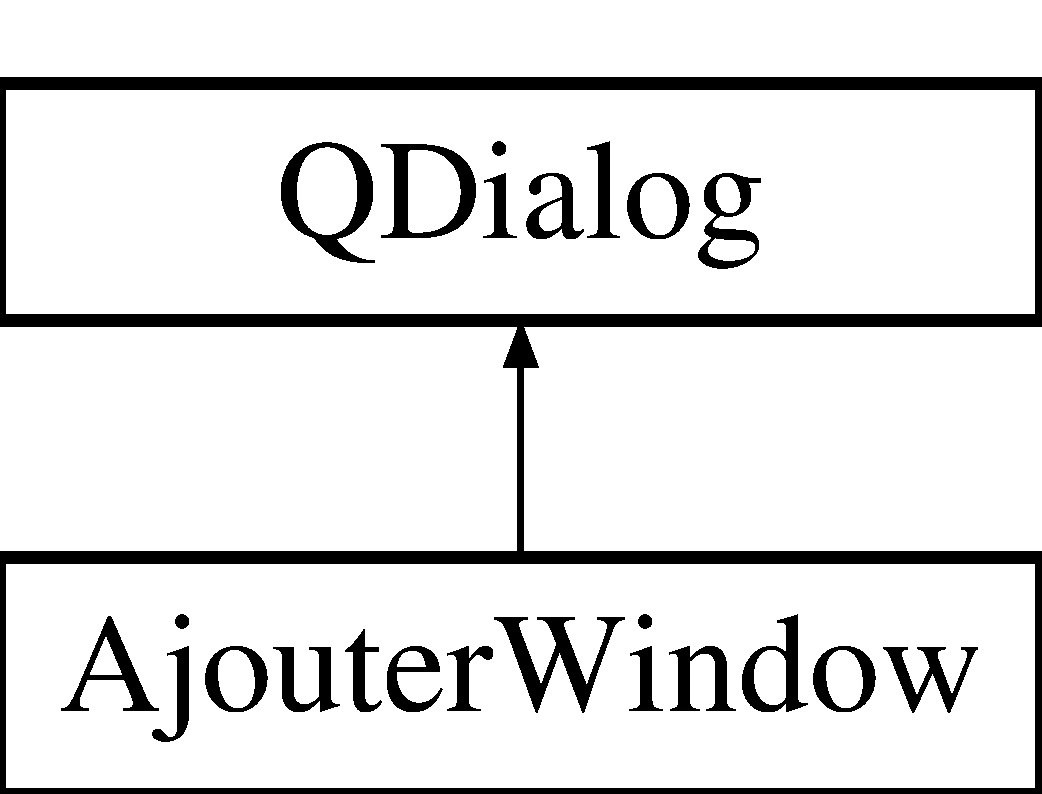
\includegraphics[height=2.000000cm]{classAjouterWindow}
\end{center}
\end{figure}
\subsection*{Public Member Functions}
\begin{DoxyCompactItemize}
\item 
\hypertarget{classAjouterWindow_a49160e34b711dab52c01c0bb9cd2fbfe}{{\bfseries Ajouter\-Window} (Q\-Widget $\ast$parent=0)}\label{classAjouterWindow_a49160e34b711dab52c01c0bb9cd2fbfe}

\item 
\hyperlink{classAction}{Action} $\ast$ \hyperlink{classAjouterWindow_a5266dae4f573c1b393d102aaeed7efc5}{get\-Action} ()
\begin{DoxyCompactList}\small\item\em get\-Action \end{DoxyCompactList}\item 
void \hyperlink{classAjouterWindow_a9a5ead98ac132e5d321b9c84b8f3e592}{charger\-Action} (\hyperlink{classAction}{Action} $\ast$a)
\begin{DoxyCompactList}\small\item\em charger\-Action \end{DoxyCompactList}\item 
void \hyperlink{classAjouterWindow_a2e29777ba09da326361a71d677a477a8}{set\-Mode} (Mode\-Fenetre\-Ajout mode)
\begin{DoxyCompactList}\small\item\em set\-Mode \end{DoxyCompactList}\item 
Mode\-Fenetre\-Ajout \hyperlink{classAjouterWindow_a2c274a0974cb2e8c02bcd47453e2a6cf}{get\-Mode} ()
\begin{DoxyCompactList}\small\item\em get\-Mode \end{DoxyCompactList}\end{DoxyCompactItemize}


\subsection{Detailed Description}
The \hyperlink{classAjouterWindow}{Ajouter\-Window} class Fenetre qui permet d'ajouter une nouvelle action ou de modifier une action existante. 

\subsection{Member Function Documentation}
\hypertarget{classAjouterWindow_a9a5ead98ac132e5d321b9c84b8f3e592}{\index{Ajouter\-Window@{Ajouter\-Window}!charger\-Action@{charger\-Action}}
\index{charger\-Action@{charger\-Action}!AjouterWindow@{Ajouter\-Window}}
\subsubsection[{charger\-Action}]{\setlength{\rightskip}{0pt plus 5cm}void Ajouter\-Window\-::charger\-Action (
\begin{DoxyParamCaption}
\item[{{\bf Action} $\ast$}]{a}
\end{DoxyParamCaption}
)}}\label{classAjouterWindow_a9a5ead98ac132e5d321b9c84b8f3e592}


charger\-Action 


\begin{DoxyParams}{Parameters}
{\em a} & Permet de charger une action déjà existante pour pouvoir la modifier \\
\hline
\end{DoxyParams}
\hypertarget{classAjouterWindow_a5266dae4f573c1b393d102aaeed7efc5}{\index{Ajouter\-Window@{Ajouter\-Window}!get\-Action@{get\-Action}}
\index{get\-Action@{get\-Action}!AjouterWindow@{Ajouter\-Window}}
\subsubsection[{get\-Action}]{\setlength{\rightskip}{0pt plus 5cm}{\bf Action} $\ast$ Ajouter\-Window\-::get\-Action (
\begin{DoxyParamCaption}
{}
\end{DoxyParamCaption}
)}}\label{classAjouterWindow_a5266dae4f573c1b393d102aaeed7efc5}


get\-Action 

\begin{DoxyReturn}{Returns}
Renvoie l'action créee ou modifiée par la fenetre 
\end{DoxyReturn}
\hypertarget{classAjouterWindow_a2c274a0974cb2e8c02bcd47453e2a6cf}{\index{Ajouter\-Window@{Ajouter\-Window}!get\-Mode@{get\-Mode}}
\index{get\-Mode@{get\-Mode}!AjouterWindow@{Ajouter\-Window}}
\subsubsection[{get\-Mode}]{\setlength{\rightskip}{0pt plus 5cm}Mode\-Fenetre\-Ajout Ajouter\-Window\-::get\-Mode (
\begin{DoxyParamCaption}
{}
\end{DoxyParamCaption}
)}}\label{classAjouterWindow_a2c274a0974cb2e8c02bcd47453e2a6cf}


get\-Mode 

\begin{DoxyReturn}{Returns}
Mode\-Fenetre\-Ajout Récupérer le mode de la fenetre 
\end{DoxyReturn}
\hypertarget{classAjouterWindow_a2e29777ba09da326361a71d677a477a8}{\index{Ajouter\-Window@{Ajouter\-Window}!set\-Mode@{set\-Mode}}
\index{set\-Mode@{set\-Mode}!AjouterWindow@{Ajouter\-Window}}
\subsubsection[{set\-Mode}]{\setlength{\rightskip}{0pt plus 5cm}void Ajouter\-Window\-::set\-Mode (
\begin{DoxyParamCaption}
\item[{Mode\-Fenetre\-Ajout}]{mode}
\end{DoxyParamCaption}
)}}\label{classAjouterWindow_a2e29777ba09da326361a71d677a477a8}


set\-Mode 


\begin{DoxyParams}{Parameters}
{\em mode} & Définit le mode de la fenetre \-: mode Ajout d'action ou ou mode Modification d'action \\
\hline
\end{DoxyParams}


The documentation for this class was generated from the following files\-:\begin{DoxyCompactItemize}
\item 
ajouterwindow.\-h\item 
ajouterwindow.\-cpp\end{DoxyCompactItemize}

\hypertarget{classAnalyseurPaquet}{\section{Analyseur\-Paquet Class Reference}
\label{classAnalyseurPaquet}\index{Analyseur\-Paquet@{Analyseur\-Paquet}}
}
\subsection*{Public Member Functions}
\begin{DoxyCompactItemize}
\item 
Type\-Paquet \hyperlink{classAnalyseurPaquet_ad9d7ab1476c2dd332b5fddfec4db0481}{reconnaitre} (Q\-String paquet)
\begin{DoxyCompactList}\small\item\em reconnaitre \end{DoxyCompactList}\end{DoxyCompactItemize}


\subsection{Member Function Documentation}
\hypertarget{classAnalyseurPaquet_ad9d7ab1476c2dd332b5fddfec4db0481}{\index{Analyseur\-Paquet@{Analyseur\-Paquet}!reconnaitre@{reconnaitre}}
\index{reconnaitre@{reconnaitre}!AnalyseurPaquet@{Analyseur\-Paquet}}
\subsubsection[{reconnaitre}]{\setlength{\rightskip}{0pt plus 5cm}Type\-Paquet Analyseur\-Paquet\-::reconnaitre (
\begin{DoxyParamCaption}
\item[{Q\-String}]{paquet}
\end{DoxyParamCaption}
)}}\label{classAnalyseurPaquet_ad9d7ab1476c2dd332b5fddfec4db0481}


reconnaitre 


\begin{DoxyParams}{Parameters}
{\em paquet} & \\
\hline
\end{DoxyParams}
\begin{DoxyReturn}{Returns}
Type de paquet A partir du paquet passé en paramètre détecte le type correspondant 
\end{DoxyReturn}


The documentation for this class was generated from the following files\-:\begin{DoxyCompactItemize}
\item 
analyseurpaquet.\-h\item 
analyseurpaquet.\-cpp\end{DoxyCompactItemize}

\hypertarget{classApprendreWindow}{\section{Apprendre\-Window Class Reference}
\label{classApprendreWindow}\index{Apprendre\-Window@{Apprendre\-Window}}
}


The \hyperlink{classApprendreWindow}{Apprendre\-Window} class Cette classe permet de choisir sur quel neurone on veut apprendre un mouvement.  




{\ttfamily \#include $<$apprendrewindow.\-h$>$}

Inheritance diagram for Apprendre\-Window\-:\begin{figure}[H]
\begin{center}
\leavevmode
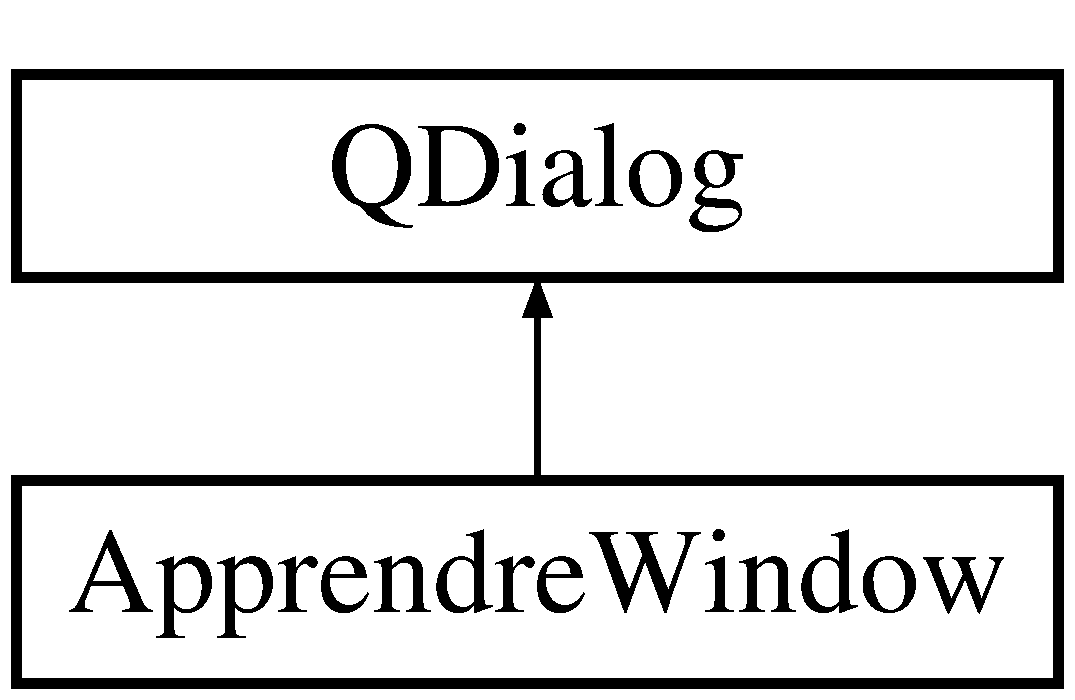
\includegraphics[height=2.000000cm]{classApprendreWindow}
\end{center}
\end{figure}
\subsection*{Public Member Functions}
\begin{DoxyCompactItemize}
\item 
\hypertarget{classApprendreWindow_a8ec93e286a2cb7363848a93d6cd74c9a}{{\bfseries Apprendre\-Window} (Q\-Widget $\ast$parent=0)}\label{classApprendreWindow_a8ec93e286a2cb7363848a93d6cd74c9a}

\item 
Q\-String \hyperlink{classApprendreWindow_a3e8a7b4d49fde43ac715db5b48302355}{get\-Commande\-Apprendre} ()
\end{DoxyCompactItemize}


\subsection{Detailed Description}
The \hyperlink{classApprendreWindow}{Apprendre\-Window} class Cette classe permet de choisir sur quel neurone on veut apprendre un mouvement. 

\subsection{Member Function Documentation}
\hypertarget{classApprendreWindow_a3e8a7b4d49fde43ac715db5b48302355}{\index{Apprendre\-Window@{Apprendre\-Window}!get\-Commande\-Apprendre@{get\-Commande\-Apprendre}}
\index{get\-Commande\-Apprendre@{get\-Commande\-Apprendre}!ApprendreWindow@{Apprendre\-Window}}
\subsubsection[{get\-Commande\-Apprendre}]{\setlength{\rightskip}{0pt plus 5cm}Q\-String Apprendre\-Window\-::get\-Commande\-Apprendre (
\begin{DoxyParamCaption}
{}
\end{DoxyParamCaption}
)}}\label{classApprendreWindow_a3e8a7b4d49fde43ac715db5b48302355}
\begin{DoxyReturn}{Returns}
la commande Permet de récupérer la commande d'aprentissage 
\end{DoxyReturn}


The documentation for this class was generated from the following files\-:\begin{DoxyCompactItemize}
\item 
apprendrewindow.\-h\item 
apprendrewindow.\-cpp\end{DoxyCompactItemize}

\hypertarget{classDevice}{\section{Device Class Reference}
\label{classDevice}\index{Device@{Device}}
}


The \hyperlink{classDevice}{Device} class.  




{\ttfamily \#include $<$device.\-h$>$}

Inheritance diagram for Device\-:\begin{figure}[H]
\begin{center}
\leavevmode
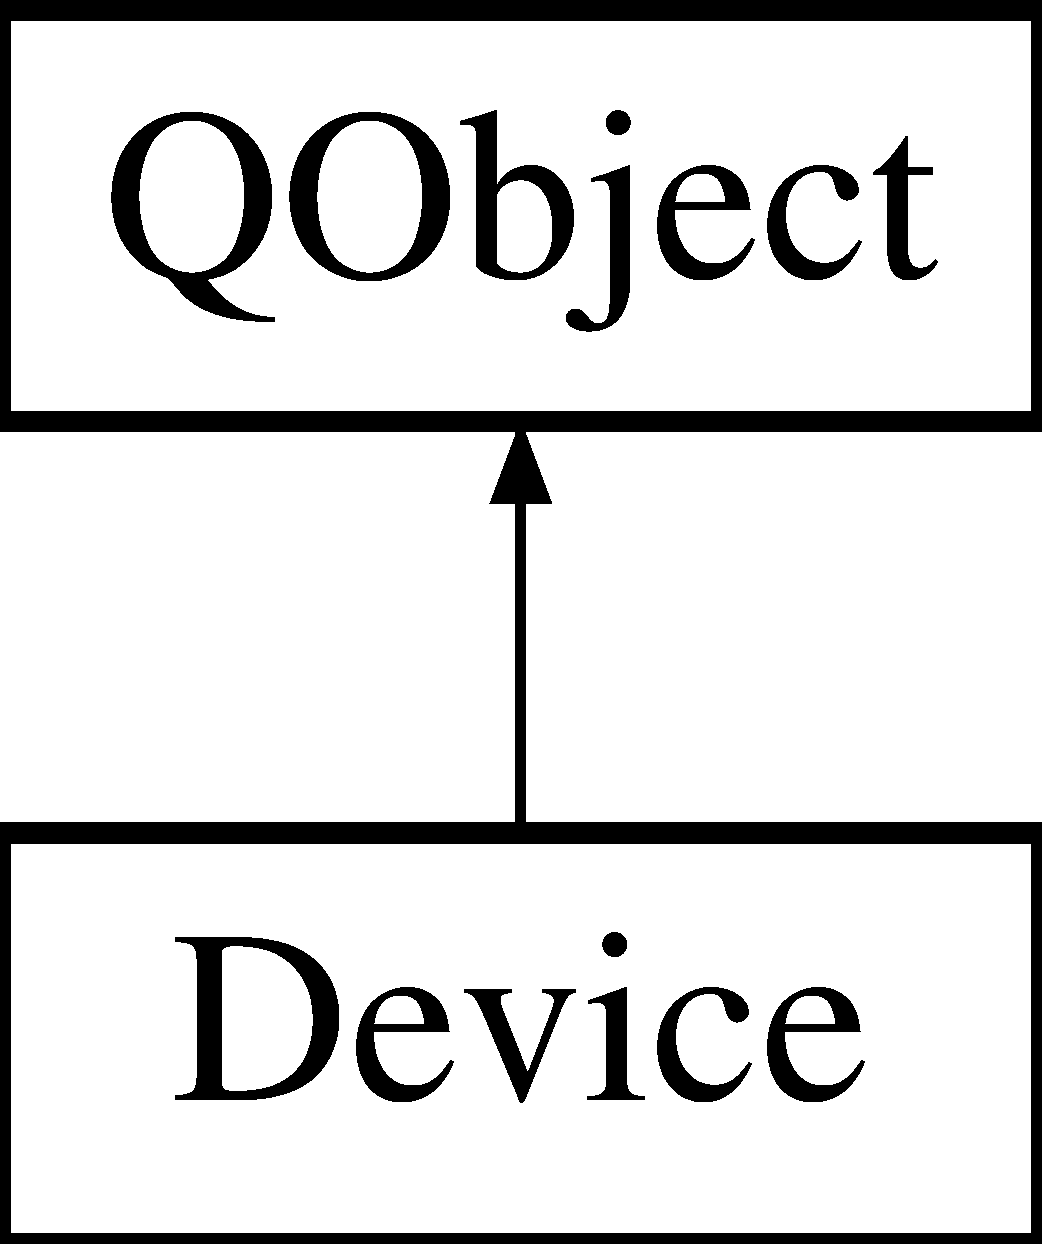
\includegraphics[height=2.000000cm]{classDevice}
\end{center}
\end{figure}
\subsection*{Public Slots}
\begin{DoxyCompactItemize}
\item 
void \hyperlink{classDevice_ae52006b42aa38769c6d30dc12c83668a}{device\-Discovered} (const Q\-Bluetooth\-Device\-Info \&device\-Info)
\begin{DoxyCompactList}\small\item\em device\-Discovered \end{DoxyCompactList}\item 
\hypertarget{classDevice_a8aa8ff0486557a7ed117766f24a077b7}{void \hyperlink{classDevice_a8aa8ff0486557a7ed117766f24a077b7}{device\-Disconnected} ()}\label{classDevice_a8aa8ff0486557a7ed117766f24a077b7}

\begin{DoxyCompactList}\small\item\em device\-Disconnected Les deconnections ne sont pas gérées pour le moment \end{DoxyCompactList}\item 
\hypertarget{classDevice_a421f7ceff3256ea79de2f316aeace553}{void \hyperlink{classDevice_a421f7ceff3256ea79de2f316aeace553}{service\-Scan\-Done} (Q\-Bluetooth\-Uuid service\-Uuid)}\label{classDevice_a421f7ceff3256ea79de2f316aeace553}

\begin{DoxyCompactList}\small\item\em service\-Scan\-Done Lorsqu'un service a été découvert, on l'identifie et on commence à chercher les informations des characteristic \end{DoxyCompactList}\item 
\hypertarget{classDevice_ac6cad0d2107e449c9027b2baf60418f2}{void \hyperlink{classDevice_ac6cad0d2107e449c9027b2baf60418f2}{device\-Connected} ()}\label{classDevice_ac6cad0d2107e449c9027b2baf60418f2}

\begin{DoxyCompactList}\small\item\em device\-Connected Lorsqu'on se connecte à un device on cherche ses services asscociés \end{DoxyCompactList}\item 
\hypertarget{classDevice_a1770e7dab50cb12e4ca64fd8c35a9eb7}{void \hyperlink{classDevice_a1770e7dab50cb12e4ca64fd8c35a9eb7}{service\-Details\-Discovered} (Q\-Low\-Energy\-Service\-::\-Service\-State)}\label{classDevice_a1770e7dab50cb12e4ca64fd8c35a9eb7}

\begin{DoxyCompactList}\small\item\em service\-Details\-Discovered Appelé quand une characteristic associé au service a été découverte, mise en place du système de notification \end{DoxyCompactList}\item 
void \hyperlink{classDevice_aab4bfb4bd87c6f38a46c88e85248978d}{position\-Characteristic\-Update} (Q\-Low\-Energy\-Characteristic ch, Q\-Byte\-Array byte\-Array)
\begin{DoxyCompactList}\small\item\em position\-Characteristic\-Update \end{DoxyCompactList}\item 
void \hyperlink{classDevice_a117df211456a907881351f34d668c272}{envoyer\-Commande} (Q\-String commande)
\begin{DoxyCompactList}\small\item\em envoyer\-Commande \end{DoxyCompactList}\item 
int \hyperlink{classDevice_aeba9db522dae3a0b46314c9ecd4bccb8}{get\-Temps\-Ecoule} ()
\end{DoxyCompactItemize}
\subsection*{Signals}
\begin{DoxyCompactItemize}
\item 
\hypertarget{classDevice_a4a90c926fc9b522a38ee0d2fdf4568a9}{void \hyperlink{classDevice_a4a90c926fc9b522a38ee0d2fdf4568a9}{maj\-Values} (float, float, float, float, float, float, float, float, float, float)}\label{classDevice_a4a90c926fc9b522a38ee0d2fdf4568a9}

\begin{DoxyCompactList}\small\item\em maj\-Values Signal émis lorsque l'on veut envoyer les données à Processing, dans l'ordre \-: yaw,ax,ay,az,vx,vy,vz,px,py,pz \end{DoxyCompactList}\item 
\hypertarget{classDevice_a6d7cf166a67336a048ddc945a9bbc7c9}{void \hyperlink{classDevice_a6d7cf166a67336a048ddc945a9bbc7c9}{maj\-Reconaissance} (int)}\label{classDevice_a6d7cf166a67336a048ddc945a9bbc7c9}

\begin{DoxyCompactList}\small\item\em maj\-Reconaissance Signal émis lors de la reconaisse d'un mouvement, le paramètre contient le numéro de mouvement / neurone \end{DoxyCompactList}\end{DoxyCompactItemize}
\subsection*{Public Member Functions}
\begin{DoxyCompactItemize}
\item 
\hypertarget{classDevice_a25d44dc002f2608a0267e895241f503e}{void {\bfseries scan} ()}\label{classDevice_a25d44dc002f2608a0267e895241f503e}

\item 
void \hyperlink{classDevice_a673451e545fc673395ffe2a5420711d1}{decouper\-Paquet} (Q\-String paquets)
\begin{DoxyCompactList}\small\item\em decouper\-Paquet \end{DoxyCompactList}\end{DoxyCompactItemize}


\subsection{Detailed Description}
The \hyperlink{classDevice}{Device} class. 

\begin{DoxyRefDesc}{Todo}
\item[\hyperlink{todo__todo000002}{Todo}]Mise à jour du rssi en temps réel Cette classe permet de scanner les devices B\-L\-E \end{DoxyRefDesc}


\subsection{Member Function Documentation}
\hypertarget{classDevice_a673451e545fc673395ffe2a5420711d1}{\index{Device@{Device}!decouper\-Paquet@{decouper\-Paquet}}
\index{decouper\-Paquet@{decouper\-Paquet}!Device@{Device}}
\subsubsection[{decouper\-Paquet}]{\setlength{\rightskip}{0pt plus 5cm}void Device\-::decouper\-Paquet (
\begin{DoxyParamCaption}
\item[{Q\-String}]{paquets}
\end{DoxyParamCaption}
)}}\label{classDevice_a673451e545fc673395ffe2a5420711d1}


decouper\-Paquet 


\begin{DoxyParams}{Parameters}
{\em paquets} & Decoupe les paquets recues en fonction de leur type et réalise les traitements liés \\
\hline
\end{DoxyParams}
\hypertarget{classDevice_ae52006b42aa38769c6d30dc12c83668a}{\index{Device@{Device}!device\-Discovered@{device\-Discovered}}
\index{device\-Discovered@{device\-Discovered}!Device@{Device}}
\subsubsection[{device\-Discovered}]{\setlength{\rightskip}{0pt plus 5cm}void Device\-::device\-Discovered (
\begin{DoxyParamCaption}
\item[{const Q\-Bluetooth\-Device\-Info \&}]{device\-Info}
\end{DoxyParamCaption}
)\hspace{0.3cm}{\ttfamily [slot]}}}\label{classDevice_ae52006b42aa38769c6d30dc12c83668a}


device\-Discovered 


\begin{DoxyParams}{Parameters}
{\em device\-Info} & Permet de traiter un device chaque fois qu'on en detecte un Lorsque le device que l'on cherchait a été trouvé, on arrete le scan et on se connecte au device \\
\hline
\end{DoxyParams}
\hypertarget{classDevice_a117df211456a907881351f34d668c272}{\index{Device@{Device}!envoyer\-Commande@{envoyer\-Commande}}
\index{envoyer\-Commande@{envoyer\-Commande}!Device@{Device}}
\subsubsection[{envoyer\-Commande}]{\setlength{\rightskip}{0pt plus 5cm}void Device\-::envoyer\-Commande (
\begin{DoxyParamCaption}
\item[{Q\-String}]{commande}
\end{DoxyParamCaption}
)\hspace{0.3cm}{\ttfamily [slot]}}}\label{classDevice_a117df211456a907881351f34d668c272}


envoyer\-Commande 


\begin{DoxyParams}{Parameters}
{\em commande} & Envoyer une commande au robot par Bluetooth en utilisant la characteristic correspondant à key\-Ch2 \\
\hline
\end{DoxyParams}
\hypertarget{classDevice_aeba9db522dae3a0b46314c9ecd4bccb8}{\index{Device@{Device}!get\-Temps\-Ecoule@{get\-Temps\-Ecoule}}
\index{get\-Temps\-Ecoule@{get\-Temps\-Ecoule}!Device@{Device}}
\subsubsection[{get\-Temps\-Ecoule}]{\setlength{\rightskip}{0pt plus 5cm}int Device\-::get\-Temps\-Ecoule (
\begin{DoxyParamCaption}
{}
\end{DoxyParamCaption}
)\hspace{0.3cm}{\ttfamily [slot]}}}\label{classDevice_aeba9db522dae3a0b46314c9ecd4bccb8}
\begin{DoxyReturn}{Returns}
Renvoie le temps écoulé depuis le lancement de l'application Chaque point sur le graphe sera associé à un temps 
\end{DoxyReturn}
\hypertarget{classDevice_aab4bfb4bd87c6f38a46c88e85248978d}{\index{Device@{Device}!position\-Characteristic\-Update@{position\-Characteristic\-Update}}
\index{position\-Characteristic\-Update@{position\-Characteristic\-Update}!Device@{Device}}
\subsubsection[{position\-Characteristic\-Update}]{\setlength{\rightskip}{0pt plus 5cm}void Device\-::position\-Characteristic\-Update (
\begin{DoxyParamCaption}
\item[{Q\-Low\-Energy\-Characteristic}]{ch, }
\item[{Q\-Byte\-Array}]{byte\-Array}
\end{DoxyParamCaption}
)\hspace{0.3cm}{\ttfamily [slot]}}}\label{classDevice_aab4bfb4bd87c6f38a46c88e85248978d}


position\-Characteristic\-Update 


\begin{DoxyParams}{Parameters}
{\em ch} & \\
\hline
{\em byte\-Array} & Methode qui permet de traiter les données recues quand on recoit une notification \\
\hline
\end{DoxyParams}


The documentation for this class was generated from the following files\-:\begin{DoxyCompactItemize}
\item 
device.\-h\item 
device.\-cpp\end{DoxyCompactItemize}

\hypertarget{classDeviceScanner}{\section{Device\-Scanner Class Reference}
\label{classDeviceScanner}\index{Device\-Scanner@{Device\-Scanner}}
}


The \hyperlink{classDeviceScanner}{Device\-Scanner} class.  




{\ttfamily \#include $<$devicescanner.\-h$>$}

Inheritance diagram for Device\-Scanner\-:\begin{figure}[H]
\begin{center}
\leavevmode
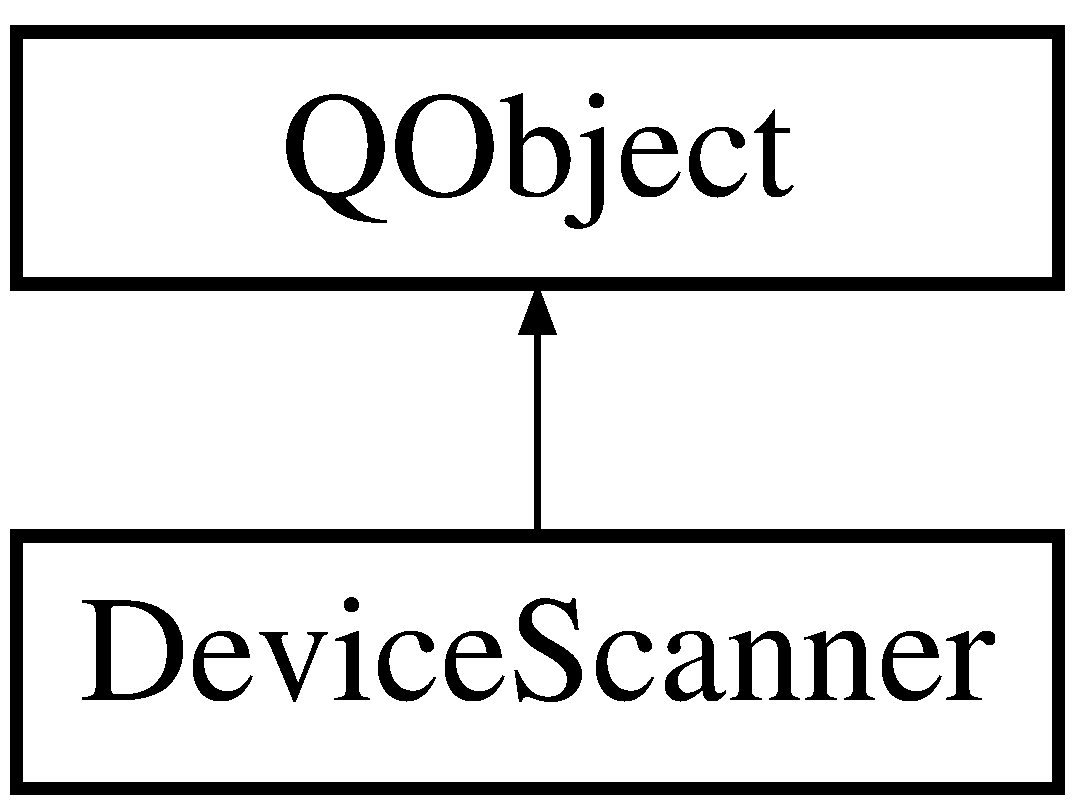
\includegraphics[height=2.000000cm]{classDeviceScanner}
\end{center}
\end{figure}
\subsection*{Public Slots}
\begin{DoxyCompactItemize}
\item 
\hypertarget{classDeviceScanner_ab7b6f00bb3e8ab9d7f1574c3d99224e6}{void {\bfseries device\-Discovered} (Q\-Bluetooth\-Device\-Info device\-Info)}\label{classDeviceScanner_ab7b6f00bb3e8ab9d7f1574c3d99224e6}

\end{DoxyCompactItemize}
\subsection*{Signals}
\begin{DoxyCompactItemize}
\item 
\hypertarget{classDeviceScanner_ab8859ba2a401533207d3ae57ee11d1e8}{void {\bfseries rssi\-Ready} (int rssi)}\label{classDeviceScanner_ab8859ba2a401533207d3ae57ee11d1e8}

\end{DoxyCompactItemize}
\subsection*{Public Member Functions}
\begin{DoxyCompactItemize}
\item 
\hypertarget{classDeviceScanner_a9e1d9f474e82601f7eb2af132122c3a3}{{\bfseries Device\-Scanner} (Q\-Bluetooth\-Device\-Discovery\-Agent $\ast$discovery\-Agent, Q\-Object $\ast$parent=0)}\label{classDeviceScanner_a9e1d9f474e82601f7eb2af132122c3a3}

\item 
\hypertarget{classDeviceScanner_a9c2367a3b9402e2a86629e2ad4fe43b9}{int {\bfseries get\-Rssi} ()}\label{classDeviceScanner_a9c2367a3b9402e2a86629e2ad4fe43b9}

\item 
\hypertarget{classDeviceScanner_aa2b766edd46ce02861a1e9a65bfb2424}{void {\bfseries run} ()}\label{classDeviceScanner_aa2b766edd46ce02861a1e9a65bfb2424}

\end{DoxyCompactItemize}


\subsection{Detailed Description}
The \hyperlink{classDeviceScanner}{Device\-Scanner} class. 

\begin{DoxyRefDesc}{Deprecated}
\item[\hyperlink{deprecated__deprecated000001}{Deprecated}]Effectuer un nouveau scan pour mettre à jour le rssi est lent et nécessite d'être déconnecté \end{DoxyRefDesc}


The documentation for this class was generated from the following files\-:\begin{DoxyCompactItemize}
\item 
devicescanner.\-h\item 
devicescanner.\-cpp\end{DoxyCompactItemize}

\hypertarget{classFile}{\section{File Class Reference}
\label{classFile}\index{File@{File}}
}
\subsection*{Public Member Functions}
\begin{DoxyCompactItemize}
\item 
\hypertarget{classFile_ad6189c0470b40e93492c27b51cce55c7}{{\bfseries File} (Q\-S)}\label{classFile_ad6189c0470b40e93492c27b51cce55c7}

\end{DoxyCompactItemize}


The documentation for this class was generated from the following files\-:\begin{DoxyCompactItemize}
\item 
file.\-h\item 
file.\-cpp\end{DoxyCompactItemize}

\hypertarget{classLineChart}{\section{Line\-Chart Class Reference}
\label{classLineChart}\index{Line\-Chart@{Line\-Chart}}
}


The \hyperlink{classLineChart}{Line\-Chart} class Cette classe contient plusieurs séries de données et peut en afficher certaines ou les cacher sur le graphique.  




{\ttfamily \#include $<$linechart.\-h$>$}

Inheritance diagram for Line\-Chart\-:\begin{figure}[H]
\begin{center}
\leavevmode
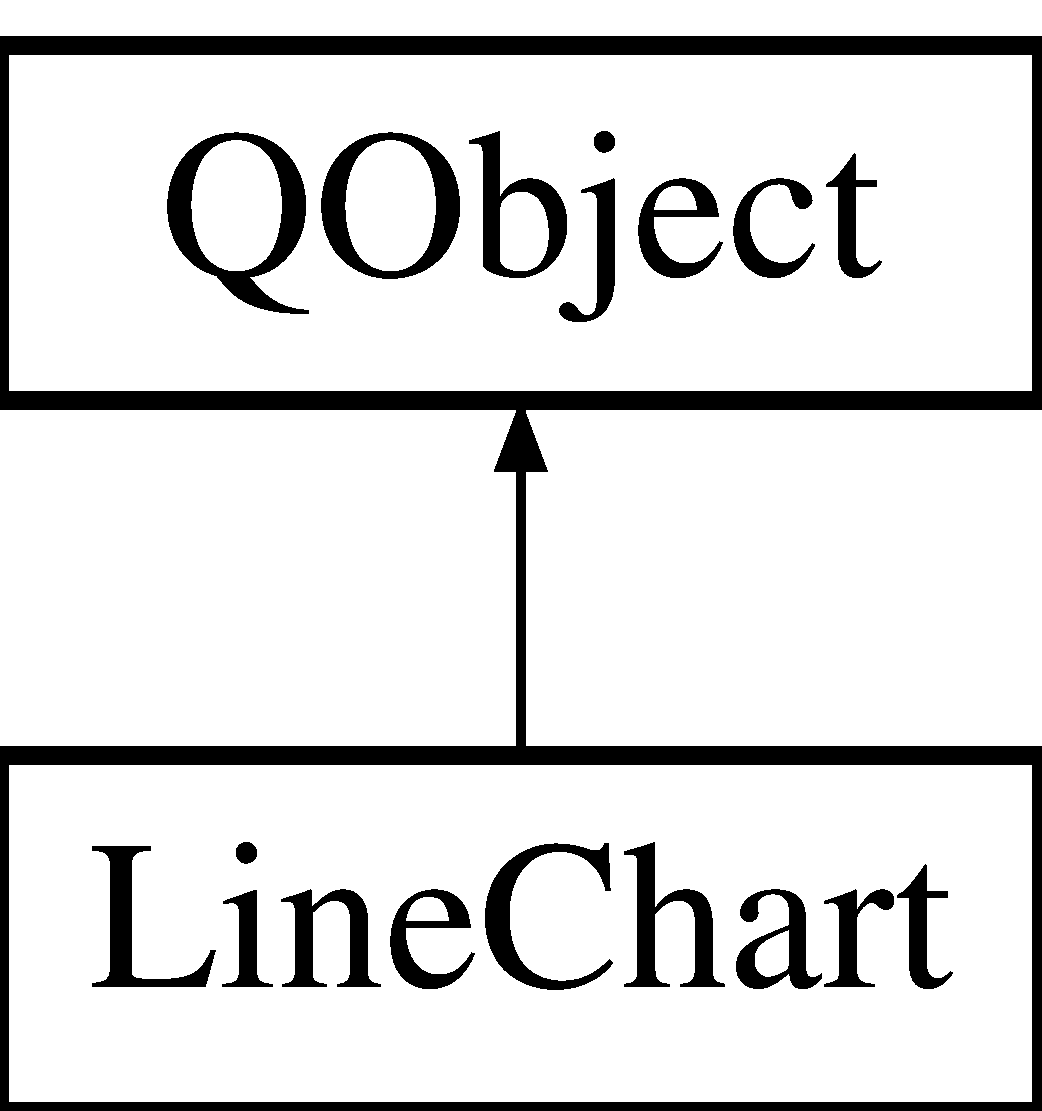
\includegraphics[height=2.000000cm]{classLineChart}
\end{center}
\end{figure}
\subsection*{Public Slots}
\begin{DoxyCompactItemize}
\item 
void \hyperlink{classLineChart_a63ff5fee1da8841e5959340669171393}{afficher\-Serie} (Q\-String nom\-Serie=\char`\"{}\char`\"{}, bool etat=false)
\item 
void \hyperlink{classLineChart_aeb7e88d90e0f6d4b52a9666839d50c35}{afficher\-Chart} ()
\item 
Q\-Color \hyperlink{classLineChart_a54618e9127e50edb4dbbbb269d422b0b}{get\-Color} (Q\-String nom\-Serie)
\item 
void \hyperlink{classLineChart_a4e468707e84690bd16a7d2b67485e745}{ajouter\-Point} (Q\-String nom\-Serie, Q\-Point\-F p)
\end{DoxyCompactItemize}
\subsection*{Public Member Functions}
\begin{DoxyCompactItemize}
\item 
\hyperlink{classSerie}{Serie} $\ast$ \hyperlink{classLineChart_add6b4014bd10e5e703f34901c305870a}{creer\-Serie} (Q\-String nom\-Serie)
\item 
Q\-Widget $\ast$ \hyperlink{classLineChart_a2e8faf97bbbb4dd5b8f50039725ce26d}{get\-View} ()
\end{DoxyCompactItemize}


\subsection{Detailed Description}
The \hyperlink{classLineChart}{Line\-Chart} class Cette classe contient plusieurs séries de données et peut en afficher certaines ou les cacher sur le graphique. 

\subsection{Member Function Documentation}
\hypertarget{classLineChart_aeb7e88d90e0f6d4b52a9666839d50c35}{\index{Line\-Chart@{Line\-Chart}!afficher\-Chart@{afficher\-Chart}}
\index{afficher\-Chart@{afficher\-Chart}!LineChart@{Line\-Chart}}
\subsubsection[{afficher\-Chart}]{\setlength{\rightskip}{0pt plus 5cm}void Line\-Chart\-::afficher\-Chart (
\begin{DoxyParamCaption}
{}
\end{DoxyParamCaption}
)\hspace{0.3cm}{\ttfamily [slot]}}}\label{classLineChart_aeb7e88d90e0f6d4b52a9666839d50c35}
Met à jour le graphe \hypertarget{classLineChart_a63ff5fee1da8841e5959340669171393}{\index{Line\-Chart@{Line\-Chart}!afficher\-Serie@{afficher\-Serie}}
\index{afficher\-Serie@{afficher\-Serie}!LineChart@{Line\-Chart}}
\subsubsection[{afficher\-Serie}]{\setlength{\rightskip}{0pt plus 5cm}void Line\-Chart\-::afficher\-Serie (
\begin{DoxyParamCaption}
\item[{Q\-String}]{nom\-Serie = {\ttfamily \char`\"{}\char`\"{}}, }
\item[{bool}]{etat = {\ttfamily false}}
\end{DoxyParamCaption}
)\hspace{0.3cm}{\ttfamily [slot]}}}\label{classLineChart_a63ff5fee1da8841e5959340669171393}

\begin{DoxyParams}{Parameters}
{\em nom\-Serie} & \\
\hline
{\em etat} & Permet de choisir si une série doit êter affichée sur le graphe ou non \\
\hline
\end{DoxyParams}
\hypertarget{classLineChart_a4e468707e84690bd16a7d2b67485e745}{\index{Line\-Chart@{Line\-Chart}!ajouter\-Point@{ajouter\-Point}}
\index{ajouter\-Point@{ajouter\-Point}!LineChart@{Line\-Chart}}
\subsubsection[{ajouter\-Point}]{\setlength{\rightskip}{0pt plus 5cm}void Line\-Chart\-::ajouter\-Point (
\begin{DoxyParamCaption}
\item[{Q\-String}]{nom\-Serie, }
\item[{Q\-Point\-F}]{p}
\end{DoxyParamCaption}
)\hspace{0.3cm}{\ttfamily [slot]}}}\label{classLineChart_a4e468707e84690bd16a7d2b67485e745}

\begin{DoxyParams}{Parameters}
{\em nom\-Serie} & \\
\hline
{\em p} & Ajoute un point à une série \\
\hline
\end{DoxyParams}
\hypertarget{classLineChart_add6b4014bd10e5e703f34901c305870a}{\index{Line\-Chart@{Line\-Chart}!creer\-Serie@{creer\-Serie}}
\index{creer\-Serie@{creer\-Serie}!LineChart@{Line\-Chart}}
\subsubsection[{creer\-Serie}]{\setlength{\rightskip}{0pt plus 5cm}{\bf Serie} $\ast$ Line\-Chart\-::creer\-Serie (
\begin{DoxyParamCaption}
\item[{Q\-String}]{nom\-Serie}
\end{DoxyParamCaption}
)}}\label{classLineChart_add6b4014bd10e5e703f34901c305870a}

\begin{DoxyParams}{Parameters}
{\em nom\-Serie} & \\
\hline
\end{DoxyParams}
\begin{DoxyReturn}{Returns}
la série créee Permet de créer une nouvelle série 
\end{DoxyReturn}
\hypertarget{classLineChart_a54618e9127e50edb4dbbbb269d422b0b}{\index{Line\-Chart@{Line\-Chart}!get\-Color@{get\-Color}}
\index{get\-Color@{get\-Color}!LineChart@{Line\-Chart}}
\subsubsection[{get\-Color}]{\setlength{\rightskip}{0pt plus 5cm}Q\-Color Line\-Chart\-::get\-Color (
\begin{DoxyParamCaption}
\item[{Q\-String}]{nom\-Serie}
\end{DoxyParamCaption}
)\hspace{0.3cm}{\ttfamily [slot]}}}\label{classLineChart_a54618e9127e50edb4dbbbb269d422b0b}

\begin{DoxyParams}{Parameters}
{\em nom\-Serie} & \\
\hline
\end{DoxyParams}
\begin{DoxyReturn}{Returns}
color Renvoie la couleur associée à une série 
\end{DoxyReturn}
\hypertarget{classLineChart_a2e8faf97bbbb4dd5b8f50039725ce26d}{\index{Line\-Chart@{Line\-Chart}!get\-View@{get\-View}}
\index{get\-View@{get\-View}!LineChart@{Line\-Chart}}
\subsubsection[{get\-View}]{\setlength{\rightskip}{0pt plus 5cm}Q\-Widget $\ast$ Line\-Chart\-::get\-View (
\begin{DoxyParamCaption}
{}
\end{DoxyParamCaption}
)}}\label{classLineChart_a2e8faf97bbbb4dd5b8f50039725ce26d}
\begin{DoxyReturn}{Returns}
view Renvoie la vue associée au graphe 
\end{DoxyReturn}


The documentation for this class was generated from the following files\-:\begin{DoxyCompactItemize}
\item 
linechart.\-h\item 
linechart.\-cpp\end{DoxyCompactItemize}

\hypertarget{classMainWindow}{\section{Main\-Window Class Reference}
\label{classMainWindow}\index{Main\-Window@{Main\-Window}}
}


The \hyperlink{classMainWindow}{Main\-Window} class Représente la fenêtre principale de l'application, elle permet d'interagir avec le robot.  




{\ttfamily \#include $<$mainwindow.\-h$>$}

Inheritance diagram for Main\-Window\-:\begin{figure}[H]
\begin{center}
\leavevmode
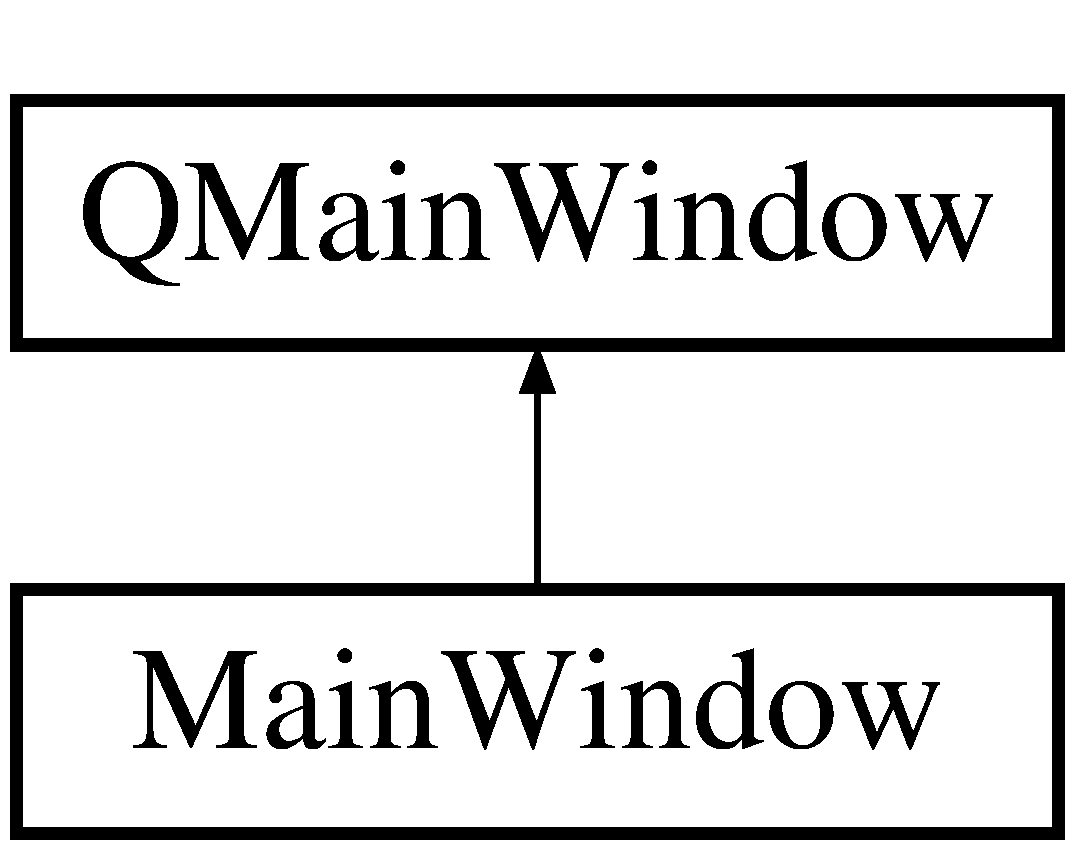
\includegraphics[height=2.000000cm]{classMainWindow}
\end{center}
\end{figure}
\subsection*{Public Member Functions}
\begin{DoxyCompactItemize}
\item 
\hypertarget{classMainWindow_a14be979a081e12f49bd8d62986d6d65e}{{\bfseries Main\-Window} (\hyperlink{classDevice}{Device} $\ast$d, Q\-Widget $\ast$parent=0)}\label{classMainWindow_a14be979a081e12f49bd8d62986d6d65e}

\end{DoxyCompactItemize}


\subsection{Detailed Description}
The \hyperlink{classMainWindow}{Main\-Window} class Représente la fenêtre principale de l'application, elle permet d'interagir avec le robot. 

The documentation for this class was generated from the following files\-:\begin{DoxyCompactItemize}
\item 
mainwindow.\-h\item 
mainwindow.\-cpp\end{DoxyCompactItemize}

\hypertarget{classMouvement}{\section{Mouvement Class Reference}
\label{classMouvement}\index{Mouvement@{Mouvement}}
}


The \hyperlink{classMouvement}{Mouvement} class La classe mouvement contient un ensemble d'actions.  




{\ttfamily \#include $<$mouvement.\-h$>$}

Inheritance diagram for Mouvement\-:\begin{figure}[H]
\begin{center}
\leavevmode
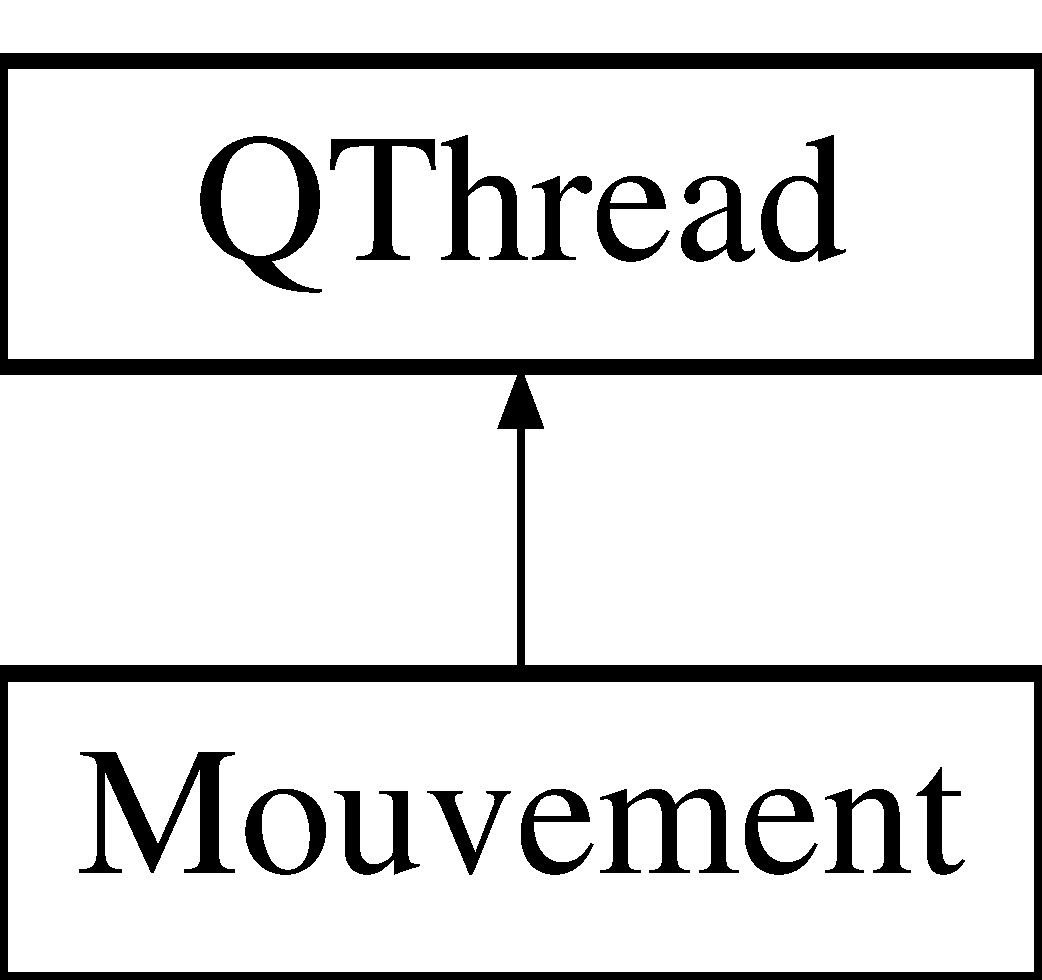
\includegraphics[height=2.000000cm]{classMouvement}
\end{center}
\end{figure}
\subsection*{Public Member Functions}
\begin{DoxyCompactItemize}
\item 
\hypertarget{classMouvement_ac8c8eb03f052b7c87acd6c8bb58d8d9f}{{\bfseries Mouvement} (\hyperlink{classDevice}{Device} $\ast$d, Q\-Object $\ast$parent)}\label{classMouvement_ac8c8eb03f052b7c87acd6c8bb58d8d9f}

\item 
void \hyperlink{classMouvement_ab2a86d3b0e1442b9cf8d1eb635ae6fe7}{ajouter\-Action} (\hyperlink{classAction}{Action} $\ast$a)
\begin{DoxyCompactList}\small\item\em ajouter\-Action \end{DoxyCompactList}\item 
void \hyperlink{classMouvement_a625b3ae43debd9411635398ce1ca17c3}{supprimer\-Action} (int id\-Action)
\begin{DoxyCompactList}\small\item\em supprimer\-Action \end{DoxyCompactList}\item 
\hypertarget{classMouvement_a00406ae24f6814b7f7ebe4601b32e1ee}{void \hyperlink{classMouvement_a00406ae24f6814b7f7ebe4601b32e1ee}{run} ()}\label{classMouvement_a00406ae24f6814b7f7ebe4601b32e1ee}

\begin{DoxyCompactList}\small\item\em run Execute le mouvement, toutes les actions qui le compose sont éxécutées les unes après les autres en respectant le délai lié à chaque action \end{DoxyCompactList}\end{DoxyCompactItemize}


\subsection{Detailed Description}
The \hyperlink{classMouvement}{Mouvement} class La classe mouvement contient un ensemble d'actions. 

\subsection{Member Function Documentation}
\hypertarget{classMouvement_ab2a86d3b0e1442b9cf8d1eb635ae6fe7}{\index{Mouvement@{Mouvement}!ajouter\-Action@{ajouter\-Action}}
\index{ajouter\-Action@{ajouter\-Action}!Mouvement@{Mouvement}}
\subsubsection[{ajouter\-Action}]{\setlength{\rightskip}{0pt plus 5cm}void Mouvement\-::ajouter\-Action (
\begin{DoxyParamCaption}
\item[{{\bf Action} $\ast$}]{a}
\end{DoxyParamCaption}
)}}\label{classMouvement_ab2a86d3b0e1442b9cf8d1eb635ae6fe7}


ajouter\-Action 


\begin{DoxyParams}{Parameters}
{\em a} & L'action à ajouter au mouvement Permet d'ajouter une nouvelle action au mouvement \\
\hline
\end{DoxyParams}
\hypertarget{classMouvement_a625b3ae43debd9411635398ce1ca17c3}{\index{Mouvement@{Mouvement}!supprimer\-Action@{supprimer\-Action}}
\index{supprimer\-Action@{supprimer\-Action}!Mouvement@{Mouvement}}
\subsubsection[{supprimer\-Action}]{\setlength{\rightskip}{0pt plus 5cm}void Mouvement\-::supprimer\-Action (
\begin{DoxyParamCaption}
\item[{int}]{id\-Action}
\end{DoxyParamCaption}
)}}\label{classMouvement_a625b3ae43debd9411635398ce1ca17c3}


supprimer\-Action 


\begin{DoxyParams}{Parameters}
{\em id\-Action} & Supprimer une action à partir de l'id de l'action dans la liste des actions du mouvement \\
\hline
\end{DoxyParams}


The documentation for this class was generated from the following files\-:\begin{DoxyCompactItemize}
\item 
mouvement.\-h\item 
mouvement.\-cpp\end{DoxyCompactItemize}

\hypertarget{classSerie}{\section{Serie Class Reference}
\label{classSerie}\index{Serie@{Serie}}
}


The \hyperlink{classSerie}{Serie} class Les séries sont prévues pour être affichés sur un Q\-Chart, elles contiennent une listes de points.  




{\ttfamily \#include $<$serie.\-h$>$}

\subsection*{Public Slots}
\begin{DoxyCompactItemize}
\item 
void \hyperlink{classSerie_a246c3b04192bc305d52ffc81ac5340fc}{ajouter\-Point} (Q\-Point\-F p)
\end{DoxyCompactItemize}
\subsection*{Public Member Functions}
\begin{DoxyCompactItemize}
\item 
\hypertarget{classSerie_a43a2d40ef45b06808c98dae95c191aa4}{{\bfseries Serie} (Q\-String nom)}\label{classSerie_a43a2d40ef45b06808c98dae95c191aa4}

\item 
Q\-List$<$ Q\-Point\-F $>$ \hyperlink{classSerie_a39c068d975a5c0986088cd9575958692}{get\-Liste\-Points} ()
\item 
Q\-String \hyperlink{classSerie_a0d52b14fd375bf668f847cc2a85efa0c}{get\-Nom} ()
\item 
void \hyperlink{classSerie_ae1f94a98b19a9b2c35e83b09f530c7c3}{set\-Afficher} (bool etat)
\item 
bool \hyperlink{classSerie_a7ba8cd41b2fec6c08c1b07338afead8e}{is\-Afficher} ()
\item 
void \hyperlink{classSerie_aaef3d2b7ea671910853c76f5b4a5a899}{set\-Color} (Q\-Color color)
\item 
Q\-Color \hyperlink{classSerie_a85bc1294501423c0b252b0b86b722609}{get\-Color} ()
\end{DoxyCompactItemize}


\subsection{Detailed Description}
The \hyperlink{classSerie}{Serie} class Les séries sont prévues pour être affichés sur un Q\-Chart, elles contiennent une listes de points. 

\subsection{Member Function Documentation}
\hypertarget{classSerie_a246c3b04192bc305d52ffc81ac5340fc}{\index{Serie@{Serie}!ajouter\-Point@{ajouter\-Point}}
\index{ajouter\-Point@{ajouter\-Point}!Serie@{Serie}}
\subsubsection[{ajouter\-Point}]{\setlength{\rightskip}{0pt plus 5cm}void Serie\-::ajouter\-Point (
\begin{DoxyParamCaption}
\item[{Q\-Point\-F}]{p}
\end{DoxyParamCaption}
)\hspace{0.3cm}{\ttfamily [slot]}}}\label{classSerie_a246c3b04192bc305d52ffc81ac5340fc}

\begin{DoxyParams}{Parameters}
{\em p} & Permet d'ajouter un point à la série \\
\hline
\end{DoxyParams}
\hypertarget{classSerie_a85bc1294501423c0b252b0b86b722609}{\index{Serie@{Serie}!get\-Color@{get\-Color}}
\index{get\-Color@{get\-Color}!Serie@{Serie}}
\subsubsection[{get\-Color}]{\setlength{\rightskip}{0pt plus 5cm}Q\-Color Serie\-::get\-Color (
\begin{DoxyParamCaption}
{}
\end{DoxyParamCaption}
)}}\label{classSerie_a85bc1294501423c0b252b0b86b722609}
\begin{DoxyReturn}{Returns}
color Renvoie la couleur associée à la série 
\end{DoxyReturn}
\hypertarget{classSerie_a39c068d975a5c0986088cd9575958692}{\index{Serie@{Serie}!get\-Liste\-Points@{get\-Liste\-Points}}
\index{get\-Liste\-Points@{get\-Liste\-Points}!Serie@{Serie}}
\subsubsection[{get\-Liste\-Points}]{\setlength{\rightskip}{0pt plus 5cm}Q\-List$<$ Q\-Point\-F $>$ Serie\-::get\-Liste\-Points (
\begin{DoxyParamCaption}
{}
\end{DoxyParamCaption}
)}}\label{classSerie_a39c068d975a5c0986088cd9575958692}
\begin{DoxyReturn}{Returns}
liste de points Renvoie la liste des points de la série 
\end{DoxyReturn}
\hypertarget{classSerie_a0d52b14fd375bf668f847cc2a85efa0c}{\index{Serie@{Serie}!get\-Nom@{get\-Nom}}
\index{get\-Nom@{get\-Nom}!Serie@{Serie}}
\subsubsection[{get\-Nom}]{\setlength{\rightskip}{0pt plus 5cm}Q\-String Serie\-::get\-Nom (
\begin{DoxyParamCaption}
{}
\end{DoxyParamCaption}
)}}\label{classSerie_a0d52b14fd375bf668f847cc2a85efa0c}
\begin{DoxyReturn}{Returns}
nom Renvoie le nom associé à la série 
\end{DoxyReturn}
\hypertarget{classSerie_a7ba8cd41b2fec6c08c1b07338afead8e}{\index{Serie@{Serie}!is\-Afficher@{is\-Afficher}}
\index{is\-Afficher@{is\-Afficher}!Serie@{Serie}}
\subsubsection[{is\-Afficher}]{\setlength{\rightskip}{0pt plus 5cm}bool Serie\-::is\-Afficher (
\begin{DoxyParamCaption}
{}
\end{DoxyParamCaption}
)}}\label{classSerie_a7ba8cd41b2fec6c08c1b07338afead8e}
\begin{DoxyReturn}{Returns}
Renvoie vrai si la série est actuellement affichée sur le graphe 
\end{DoxyReturn}
\hypertarget{classSerie_ae1f94a98b19a9b2c35e83b09f530c7c3}{\index{Serie@{Serie}!set\-Afficher@{set\-Afficher}}
\index{set\-Afficher@{set\-Afficher}!Serie@{Serie}}
\subsubsection[{set\-Afficher}]{\setlength{\rightskip}{0pt plus 5cm}void Serie\-::set\-Afficher (
\begin{DoxyParamCaption}
\item[{bool}]{etat}
\end{DoxyParamCaption}
)}}\label{classSerie_ae1f94a98b19a9b2c35e83b09f530c7c3}

\begin{DoxyParams}{Parameters}
{\em etat} & Définit si la série doit être affichée ou non \\
\hline
\end{DoxyParams}
\hypertarget{classSerie_aaef3d2b7ea671910853c76f5b4a5a899}{\index{Serie@{Serie}!set\-Color@{set\-Color}}
\index{set\-Color@{set\-Color}!Serie@{Serie}}
\subsubsection[{set\-Color}]{\setlength{\rightskip}{0pt plus 5cm}void Serie\-::set\-Color (
\begin{DoxyParamCaption}
\item[{Q\-Color}]{color}
\end{DoxyParamCaption}
)}}\label{classSerie_aaef3d2b7ea671910853c76f5b4a5a899}

\begin{DoxyParams}{Parameters}
{\em color} & Définit la couleur associé à la série \\
\hline
\end{DoxyParams}


The documentation for this class was generated from the following files\-:\begin{DoxyCompactItemize}
\item 
serie.\-h\item 
serie.\-cpp\end{DoxyCompactItemize}

\hypertarget{classTraitementDonnees}{\section{Traitement\-Donnees Class Reference}
\label{classTraitementDonnees}\index{Traitement\-Donnees@{Traitement\-Donnees}}
}


The \hyperlink{classTraitementDonnees}{Traitement\-Donnees} class.  




{\ttfamily \#include $<$traitementdonnees.\-h$>$}

\subsection*{Public Member Functions}
\begin{DoxyCompactItemize}
\item 
void \hyperlink{classTraitementDonnees_a26e84d4ff8b228448fa4341a0f626810}{set\-Acceleration} (float ax, float ay, float az)
\item 
void \hyperlink{classTraitementDonnees_aae3b3983aebcc36db7519e3d4c9defc8}{calculer\-Vitesse} ()
\item 
void \hyperlink{classTraitementDonnees_a0658a30ce0080052590f43175678b1a3}{calculer\-Position} ()
\item 
void \hyperlink{classTraitementDonnees_a47d3b55731475591334af21c15bf0faa}{mise\-A\-Jour\-Val} ()
\item 
\hypertarget{classTraitementDonnees_a7d25ee8242fd6c5e3dfa0c168a881930}{float $\ast$ {\bfseries get\-Acceleration\-Courante} ()}\label{classTraitementDonnees_a7d25ee8242fd6c5e3dfa0c168a881930}

\item 
\hypertarget{classTraitementDonnees_aa0f3af6b3031701f8500efc9d22c10db}{float $\ast$ {\bfseries get\-Vitesse\-Courante} ()}\label{classTraitementDonnees_aa0f3af6b3031701f8500efc9d22c10db}

\item 
\hypertarget{classTraitementDonnees_a97add932d94c275e7fac5682653802f7}{float $\ast$ {\bfseries get\-Position\-Courante} ()}\label{classTraitementDonnees_a97add932d94c275e7fac5682653802f7}

\item 
float \hyperlink{classTraitementDonnees_a81ffbc75f47488f0e4bbfbff13aeff0c}{get\-Roll} ()
\item 
float \hyperlink{classTraitementDonnees_ad7f0fe073028f88d5520bd30ddef0fd5}{get\-Yaw} ()
\item 
float \hyperlink{classTraitementDonnees_a0c0db9953a514fdef8c2155ea0f2555f}{get\-Pitch} ()
\item 
void \hyperlink{classTraitementDonnees_a3b399278ae62f30b2faeedf89dd26094}{traitement} (float ax, float ay, float az, float gx, float gy, float gz, bool immobile, float intervalle)
\item 
void \hyperlink{classTraitementDonnees_abae534e845da998de4cce9a23df96433}{calcul\-Quaternions} (float gx, float gy, float gz, float ax, float ay, float az)
\end{DoxyCompactItemize}


\subsection{Detailed Description}
The \hyperlink{classTraitementDonnees}{Traitement\-Donnees} class. 

\subsection{Member Function Documentation}
\hypertarget{classTraitementDonnees_a0658a30ce0080052590f43175678b1a3}{\index{Traitement\-Donnees@{Traitement\-Donnees}!calculer\-Position@{calculer\-Position}}
\index{calculer\-Position@{calculer\-Position}!TraitementDonnees@{Traitement\-Donnees}}
\subsubsection[{calculer\-Position}]{\setlength{\rightskip}{0pt plus 5cm}void Traitement\-Donnees\-::calculer\-Position (
\begin{DoxyParamCaption}
{}
\end{DoxyParamCaption}
)}}\label{classTraitementDonnees_a0658a30ce0080052590f43175678b1a3}
Calcul des positions à partir des vitesses \hypertarget{classTraitementDonnees_aae3b3983aebcc36db7519e3d4c9defc8}{\index{Traitement\-Donnees@{Traitement\-Donnees}!calculer\-Vitesse@{calculer\-Vitesse}}
\index{calculer\-Vitesse@{calculer\-Vitesse}!TraitementDonnees@{Traitement\-Donnees}}
\subsubsection[{calculer\-Vitesse}]{\setlength{\rightskip}{0pt plus 5cm}void Traitement\-Donnees\-::calculer\-Vitesse (
\begin{DoxyParamCaption}
{}
\end{DoxyParamCaption}
)}}\label{classTraitementDonnees_aae3b3983aebcc36db7519e3d4c9defc8}
Calcul des vitesses à partir des accélérations \hypertarget{classTraitementDonnees_abae534e845da998de4cce9a23df96433}{\index{Traitement\-Donnees@{Traitement\-Donnees}!calcul\-Quaternions@{calcul\-Quaternions}}
\index{calcul\-Quaternions@{calcul\-Quaternions}!TraitementDonnees@{Traitement\-Donnees}}
\subsubsection[{calcul\-Quaternions}]{\setlength{\rightskip}{0pt plus 5cm}void Traitement\-Donnees\-::calcul\-Quaternions (
\begin{DoxyParamCaption}
\item[{float}]{gx, }
\item[{float}]{gy, }
\item[{float}]{gz, }
\item[{float}]{ax, }
\item[{float}]{ay, }
\item[{float}]{az}
\end{DoxyParamCaption}
)}}\label{classTraitementDonnees_abae534e845da998de4cce9a23df96433}

\begin{DoxyParams}{Parameters}
{\em gx} & \\
\hline
{\em gy} & \\
\hline
{\em gz} & \\
\hline
{\em ax} & \\
\hline
{\em ay} & \\
\hline
{\em az} & On utilise l'algorithme de Madgwick pour calculer les quaternions roll yaw pitch à partir des 6 accélérations Les qquaternions donnent la rotation sur les 3 axes de la carte \\
\hline
\end{DoxyParams}
\hypertarget{classTraitementDonnees_a0c0db9953a514fdef8c2155ea0f2555f}{\index{Traitement\-Donnees@{Traitement\-Donnees}!get\-Pitch@{get\-Pitch}}
\index{get\-Pitch@{get\-Pitch}!TraitementDonnees@{Traitement\-Donnees}}
\subsubsection[{get\-Pitch}]{\setlength{\rightskip}{0pt plus 5cm}float Traitement\-Donnees\-::get\-Pitch (
\begin{DoxyParamCaption}
{}
\end{DoxyParamCaption}
)}}\label{classTraitementDonnees_a0c0db9953a514fdef8c2155ea0f2555f}
\begin{DoxyReturn}{Returns}
Renvoie pitch 
\end{DoxyReturn}
\hypertarget{classTraitementDonnees_a81ffbc75f47488f0e4bbfbff13aeff0c}{\index{Traitement\-Donnees@{Traitement\-Donnees}!get\-Roll@{get\-Roll}}
\index{get\-Roll@{get\-Roll}!TraitementDonnees@{Traitement\-Donnees}}
\subsubsection[{get\-Roll}]{\setlength{\rightskip}{0pt plus 5cm}float Traitement\-Donnees\-::get\-Roll (
\begin{DoxyParamCaption}
{}
\end{DoxyParamCaption}
)}}\label{classTraitementDonnees_a81ffbc75f47488f0e4bbfbff13aeff0c}
\begin{DoxyReturn}{Returns}
Renvoie roll 
\end{DoxyReturn}
\hypertarget{classTraitementDonnees_ad7f0fe073028f88d5520bd30ddef0fd5}{\index{Traitement\-Donnees@{Traitement\-Donnees}!get\-Yaw@{get\-Yaw}}
\index{get\-Yaw@{get\-Yaw}!TraitementDonnees@{Traitement\-Donnees}}
\subsubsection[{get\-Yaw}]{\setlength{\rightskip}{0pt plus 5cm}float Traitement\-Donnees\-::get\-Yaw (
\begin{DoxyParamCaption}
{}
\end{DoxyParamCaption}
)}}\label{classTraitementDonnees_ad7f0fe073028f88d5520bd30ddef0fd5}
\begin{DoxyReturn}{Returns}
Renvoie yaw 
\end{DoxyReturn}
\hypertarget{classTraitementDonnees_a47d3b55731475591334af21c15bf0faa}{\index{Traitement\-Donnees@{Traitement\-Donnees}!mise\-A\-Jour\-Val@{mise\-A\-Jour\-Val}}
\index{mise\-A\-Jour\-Val@{mise\-A\-Jour\-Val}!TraitementDonnees@{Traitement\-Donnees}}
\subsubsection[{mise\-A\-Jour\-Val}]{\setlength{\rightskip}{0pt plus 5cm}void Traitement\-Donnees\-::mise\-A\-Jour\-Val (
\begin{DoxyParamCaption}
{}
\end{DoxyParamCaption}
)}}\label{classTraitementDonnees_a47d3b55731475591334af21c15bf0faa}
Met à jour la matrice d'accélérations \hypertarget{classTraitementDonnees_a26e84d4ff8b228448fa4341a0f626810}{\index{Traitement\-Donnees@{Traitement\-Donnees}!set\-Acceleration@{set\-Acceleration}}
\index{set\-Acceleration@{set\-Acceleration}!TraitementDonnees@{Traitement\-Donnees}}
\subsubsection[{set\-Acceleration}]{\setlength{\rightskip}{0pt plus 5cm}void Traitement\-Donnees\-::set\-Acceleration (
\begin{DoxyParamCaption}
\item[{float}]{ax, }
\item[{float}]{ay, }
\item[{float}]{az}
\end{DoxyParamCaption}
)}}\label{classTraitementDonnees_a26e84d4ff8b228448fa4341a0f626810}

\begin{DoxyParams}{Parameters}
{\em ax} & \\
\hline
{\em ay} & \\
\hline
{\em az} & Définit les accélérations pour les calculs \\
\hline
\end{DoxyParams}
\hypertarget{classTraitementDonnees_a3b399278ae62f30b2faeedf89dd26094}{\index{Traitement\-Donnees@{Traitement\-Donnees}!traitement@{traitement}}
\index{traitement@{traitement}!TraitementDonnees@{Traitement\-Donnees}}
\subsubsection[{traitement}]{\setlength{\rightskip}{0pt plus 5cm}void Traitement\-Donnees\-::traitement (
\begin{DoxyParamCaption}
\item[{float}]{ax, }
\item[{float}]{ay, }
\item[{float}]{az, }
\item[{float}]{gx, }
\item[{float}]{gy, }
\item[{float}]{gz, }
\item[{bool}]{immobile, }
\item[{float}]{intervalle}
\end{DoxyParamCaption}
)}}\label{classTraitementDonnees_a3b399278ae62f30b2faeedf89dd26094}

\begin{DoxyParams}{Parameters}
{\em ax} & \\
\hline
{\em ay} & \\
\hline
{\em az} & \\
\hline
{\em gx} & \\
\hline
{\em gy} & \\
\hline
{\em gz} & \\
\hline
{\em immobile} & \\
\hline
{\em intervalle} & Permet de calculer les vitesses, positions et les quaternions \\
\hline
\end{DoxyParams}


The documentation for this class was generated from the following files\-:\begin{DoxyCompactItemize}
\item 
traitementdonnees.\-h\item 
traitementdonnees.\-cpp\end{DoxyCompactItemize}

%--- End generated contents ---

% Index
\newpage
\phantomsection
\addcontentsline{toc}{chapter}{Index}
\printindex

\end{document}
